%%%%%%%%%%%%%%%%%%%%%%%%%%%%%%%%%%%%%%%%%%%%%%%%%%%%%%%%%%
% # Appendix: Brown Cloze Test
%%%%%%%%%%%%%%%%%%%%%%%%%%%%%%%%%%%%%%%%%%%%%%%%%%%%%%%%%%

\chapter{Brown Cloze Test}\label{app-brown}

Brown's (\citeyear{brown1980}) cloze test was included in the C-test validation study. Participants were all L1-Korean L2ers of English (KLEs).

\vspace{0.5cm}

\textbf{Instructions:} (1) Read the passage quickly to get the general meaning. (2) Write \myuline{only one} word in each blank. Contractions (example: \myuline{don't}) and possessives (\myuline{John's} bicycle) are one word. \mbox{(3) Spelling} will not count against you as long as the scorer can read the word.

\vspace{0.5 cm}

\textbf{Example:} The boy walked up the street. He stepped \gap[align=left]{on} a piece of ice. He fell \gap[align=left]{down} but he didn't hurt himself.

\vspace{0.5 cm}

\begin{center} \textbf{Man and His Progress} \end{center}

\vspace{0.1 cm}
\begin{spacing}{1.2}

Man is the only living creature that can make and use tools. He is the most teachable of living beings, earning the name Homo sapiens. \gap{1} ever restless brain has used the \gap{2} and wisdom of his ancestors \gap{3} improve his way of life. Since \gap{4} is able to walk and run \gap{5} his feet, his hands have always \gap{6} free to carry and to use \gap{7}. Man's hands have served him well \gap{8} his life on earth. His development, \gap{9} can be divided into three major \gap{10}, is marked by several different ways \gap{11} life.

\vspace{0.5 cm}

Up to 10,000 years ago, \gap{12} human beings lived by hunting and \gap{13}. They also picked berries and fruits, \gap{14} dug for various edible roots. Most \gap{15}, the men were the hunters, and \gap{16} women acted as food gatherers. Since \gap{17} women were busy with the children, \gap{18} men handled the tools. In a \gap{19} hand, a dead branch became a \gap{20} to knock down fruit or to \gap{21} for tasty roots. Sometimes, an animal \gap{22} served as a club, and a \gap{23} piece of stone, fitting comfortably into \gap{24} hand, could be used to break \gap{25} or to throw at an animal. \gap{26} stone was chipped against another until \gap{27} had a sharp edge. The primitive \gap{28} who first thought of putting a \gap{29} stone at the end of a \gap{30} made a brilliant discovery: he \gap{31} joined two things to make a \gap{32} useful tool, the spear. Flint, found \gap{33} many rocks, became a common cutting \gap{34} in the Paleolithic period of man's \gap{35}. Since no wood or bone tools \gap{36} survived, we know of this man \gap{37} his stone implements, with which he \gap{38} kill animals, cut up the meat, \gap{39} scrape the skins, as well as \gap{40} pictures on the walls of the \gap{41} where he lived during the winter.

\vspace{0.5 cm}

\gap{42} the warmer seasons, man wandered on \gap{43} steppes of Europe without a fixed \gap{44}, always foraging for food. Perhaps the \gap{45} carried nuts and berries in shells \gap{46} skins or even in light, woven \gap{47}. Wherever they camped, the primitive people \gap{48} fires by striking flint for sparks \gap{49} using dried seeds, moss, and rotten \gap{50} for tinder. With fires that he kindled himself, man could keep wild animals away and could cook those that he killed, as well as provide warmth and light for himself.

\end{spacing}

\vspace{0.5 cm}

\textbf{Answers:} (1)~his man's our the, (2)~knowledge accomplishments culture cunning examples experience experiences hands ideas information ingenuity instinct intelligence mistakes nature power skill skills talent teaching technique thought will wit words work, (3)~to, (4)~man he, (5)~on upon using with, (6)~been felt hung remained, (7)~tools adequately carefully conventionally creatively diligently efficiently freely implements objects productively readily them things weapons, (8)~during all for improving in through throughout with, (9)~which also basically conveniently easily historically however often since that thus, (10)~periods areas categories divisions eras facets groups parts phases sections stages steps topics trends, (11)~of for in through towards, (12)~all early hungry many most only primitive the these, (13)~fishing farming foraging gathering killing scavenging scrounging sleeping trapping, (14)~and often ravenously some the, (15)~often always emphatically important nights normally of times trips, (16)~the all house many most older their younger, (17)~the all many married most often older primate these, (18)~the all constructive many most older primate tough younger, (19)~man's able big closed coordinated creative deft empty free human human's hunter's learned needed needy person's right single skilled skillful small strong trained, (20)~tool club device instrument pole rod spear stick weapon, (21)~dig burrow excavate probe search test, (22)~bone arm easily foot had hide horn leg skull tusk, (23)~sharp big chipped fashioned flat hard heavy large rough round shaped sizeable small smooth solid strong soft thin, (24)~the a his man's one one's, (25)~nuts apart bark bones branches coconuts down firewood food heads ice items meat objects open rocks shells sticks stone things tinder trees wood, (26)~one a each flat flint glass hard obsidian shale softer some the then this, (27)~it each one they, (28)~man being creature human's hunter men owner people person, (29)~sharp glass hard jagged large lime pointed sharpened small, (30)~stick bone branch club log pole rod shaft, (31)~had accidentally cleverly clumsily conveniently creatively dexterously double easily first ingeniously securely simply soon suddenly tastefully tightly then would, (32)~very bad extremely good hunter's incredibly intelligent long modern most necessarily new portentously quite tremendously useful, (33)~in all among amongst by inside on that using within, (34)~tool device edge implement instrument item material method objects piece practice stone utensil, (35)~development age ancestry discoveries era evolution existence exploration history life time, (36)~have actually apparently ever, (37)~by and for from had made through used using, (38)~could did would, (39)~and carefully help or skillfully then would, (40)~draw carve create drawing engrave hang paint painting place sketch some the, (41)~cave caves animals place places room, (42)~in and during with, (43)~the across aimless all barren in dry flat high long many plain stone through to toward unknown various, (44)~home appetite camp course destination destiny diet direction domain foundation habitat income knowledge location lunch map meal path pattern place plan route supplement supply time weapons, (45)~women children families group human hunter man men people primitives voyager wanderers woman, (46)~or and animal animal's covered in like often on their using with, (47)~baskets bags blankets chests cloth clothes fabric garments hides material nets pouches sacks, (48)~made began built lighted lit produced started used, (49)~and also by occasionally or then together while, (50)~wood bark branches dung forage grass leaves lumber roots skin timber tree trees

\vspace {0.5 cm}

\textit{Note}. For each set of answers, the first word is the exact answer and the rest are acceptable responses as determined by Brown [-@brown1980].

\newpage

%========================================================%
\section{Korean instructions}
%========================================================%

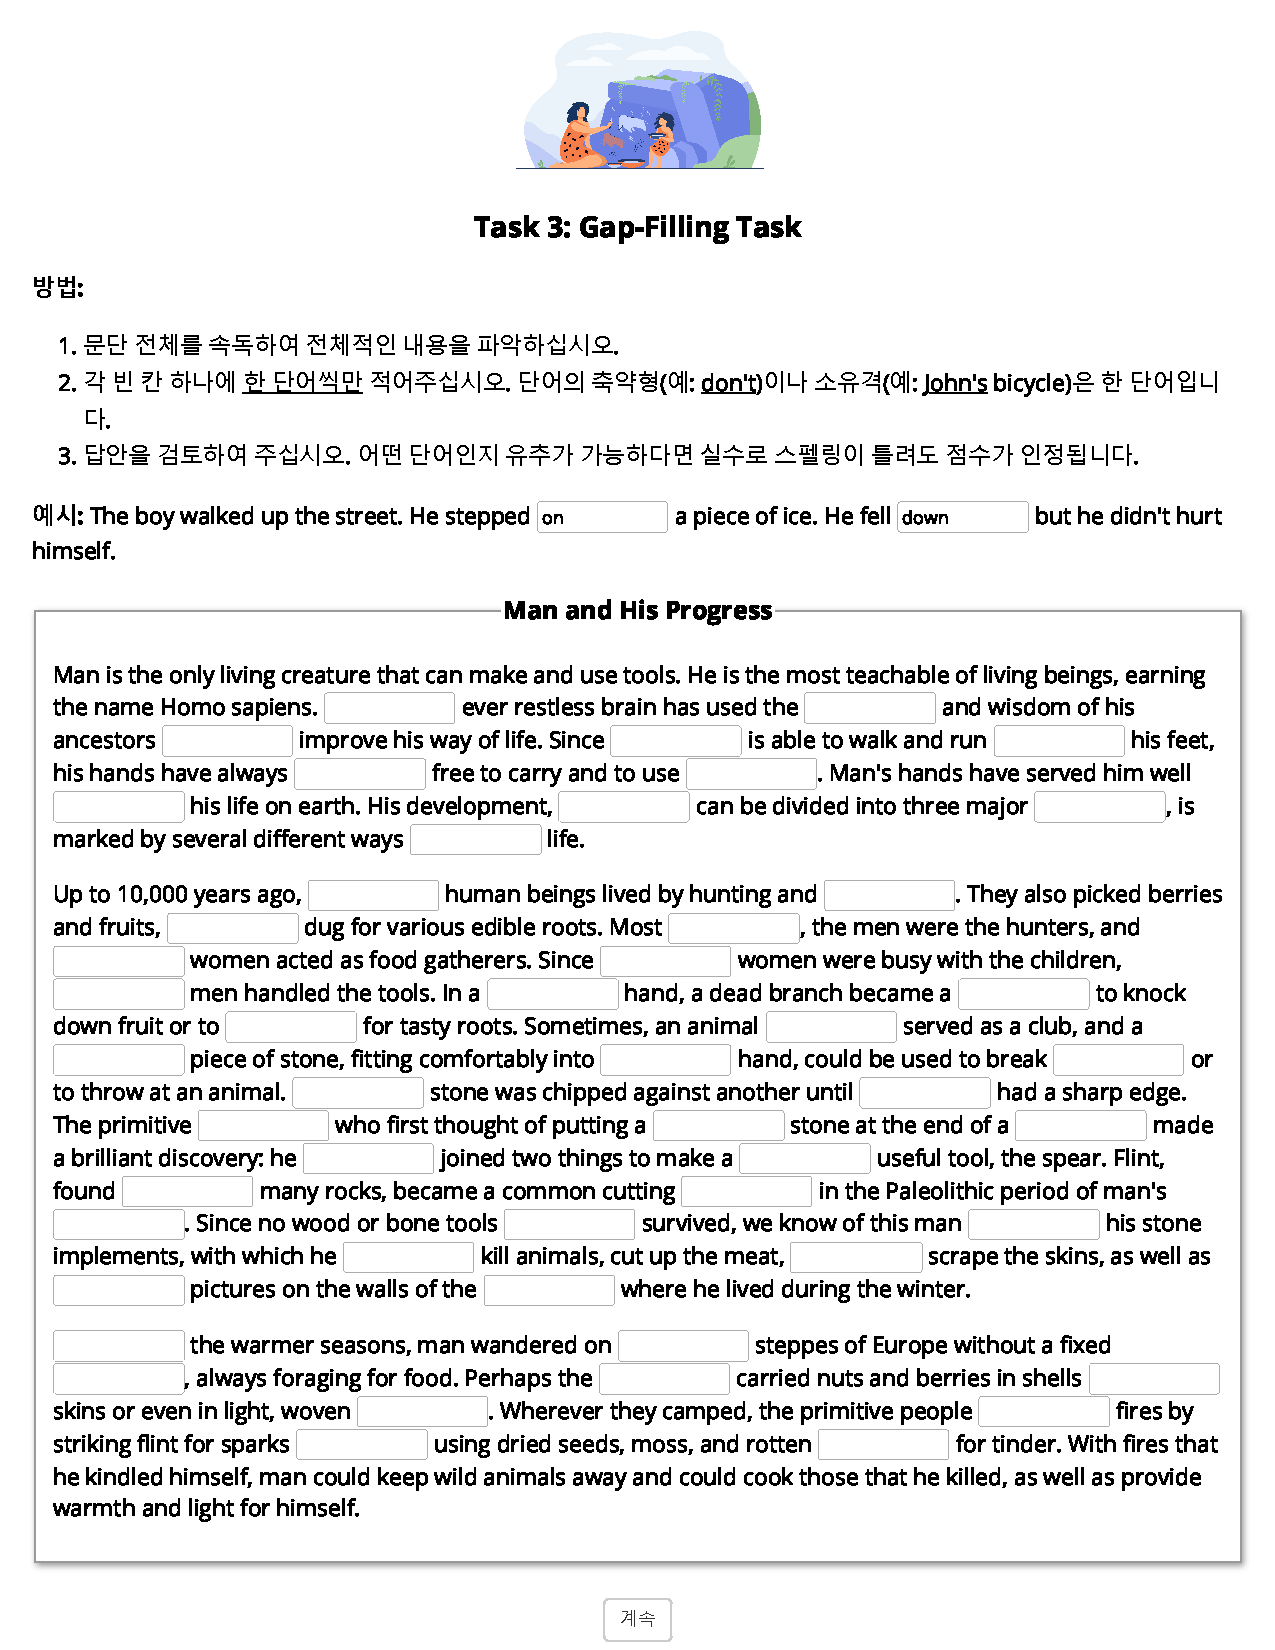
\includegraphics{../materials/instructions/ko-ct-br.pdf}